\documentclass[cal1spr16Lectures.tex]{subfiles}

\begin{document}

\section[]{}

% % %
\subsection[5.3 Fundamental Theorem of Calculus]{\S 5.3 Fundamental Theorem of Calculus}
% % %

% % %
\begin{frame}{\S 5.3 Fundamental Theorem of Calculus}
Using Riemann sums to evaluate definite integrals is usually neither efficient nor practical.  We will develop methods to evaluate integrals and also tie together the concepts of differentiation and integration. 

\vspace{0.5pc}
To connect the concepts of differention and integration, we first must define the concept of an area function.
\end{frame}

% % %
\subsubsection{Area Functions}
% % %

% % %
\begin{frame}{\small Area Functions}\footnotesize
Let $y=f(t)$ be a continuous function which is defined for all $t \ge a$, where $a$ is a fixed number.  The area function for $f$ with left endpoint at $a$ is given by 
%
%\vspace{-1.5pc}
%\[]
$A(x)=\int_a^x f(t)\ dt$.%\]  

\vspace{-1pc}
\begin{center}
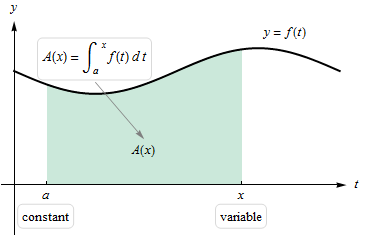
\includegraphics[scale=0.55]{pictures/Fig5_32}
\end{center}

\vspace{-1.5pc}
This gives the net area of the region between the graph of $f$ and the $t$-axis between the points $t=a$ and $t=x$.  %(See Figure 5.33 on p.\ 335 for pictures of the area function in action.) 
\end{frame}

% % %
\begin{frame}
\begin{center}
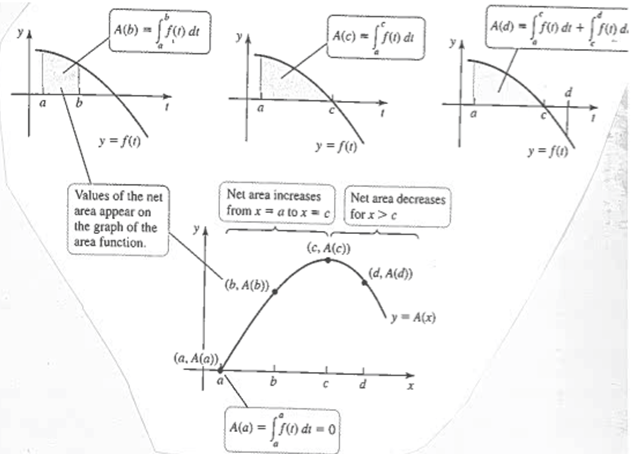
\includegraphics[scale=1.25]{pictures/5p3example}
\end{center}
\end{frame}

% % %
\begin{frame}\footnotesize
\begin{ex} 
The graph of $f$ is shown below.  Let 

\vspace{-0.75pc}
\[A(x)=\int_0^x f(t)\ dt\quad\text{ and }\quad F(x)=\int_2^x f(t)\ dt\] 

\vspace{-0.25pc}
be two area functions for $f$.  Compute $A(2), F(5), A(5), F(8)$.

\vspace{-0.65pc}
\begin{center}
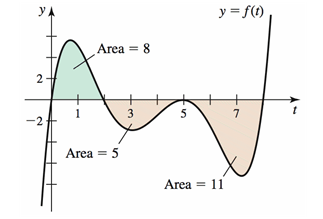
\includegraphics[scale=0.85]{pictures/Ch5Sect3_Exer12}
\end{center}
\end{ex}
\end{frame}

% % %
\subsubsection{The Fundamental Theorem of Calculus (Part 1)}
% % %

% % %
\begin{frame}{\small The Fundamental Theorem of Calculus (Part 1)}
Linear functions help to build the rationale behind the Fundamental Theorem of Calculus.
\begin{ex}
Let $f(t)=4t+3$ and define $A(x)=\int_1^xf(t)\ dt$.  What is $A(2)$? $A(4)$? $A(x)$? $A'(x)$?
\end{ex}
In general, the property illustrated with this linear function works for all continuous functions and is one part of the FTOC (Fundamental Theorem of Calculus).
\end{frame}

% % %
\begin{frame}\small
\begin{thm}[FTOC I] If $f$ is continuous on $[a,b]$, then the area function $A(x)=\int_a^x f(t)\ dt$ for $a \le x \le b$ is continuous on $[a,b]$ and differentiable on $(a,b)$.  The area function satisfies $A^{\prime}(x)=f(x)$; or equivalently, 
\[
A^{\prime}(x)=\frac{d}{dx} \int_a^x f(t)\ dt = f(x)
\]
which means that the area function of $f$ is an antiderivative of $f$.
\end{thm}
\end{frame}

% % %
\subsubsection{The Fundamental Theorem of Calculus (Part 2)}
% % %

% % %
\begin{frame}{\small The Fundamental Theorem of Calculus (Part 2)}\small
Since $A$ is an antiderivative of $f$, we now have a way to evaluate definite integrals and find areas under curves.
\begin{thm}[FTOC II] 
If $f$ is continuous on $[a,b]$ and $F$ is any antiderivative of $f$, then
\[\int_a^b f(x)\ dx = F(b)-F(a).\]
\end{thm}
%
%\vspace{1pc}
We use the notation $F(x) \vert_a^b = F(b)-F(a)$.
\end{frame}

% % %
\subsubsection{Overview of FTOC}
% % %

% % %
\begin{frame}{\small Overview of FTOC}\small
In essence, to evaluate an integral, we
\begin{itemize}
\item Find any antiderivative of $f$, and call if $F$.
\item Compute $F(b)-F(a)$, the difference in the values of $F$ between the upper and lower limits of integration.
\end{itemize}
The two parts of the FTOC illustrate the inverse relationship between differentiation and integration -- the integral ``undoes'' the derivative.
\end{frame}

% % %
\begin{frame}
\begin{ex}
\begin{itemize}\small
\item[(1)] Use Part 1 of the FTOC to simplify $\displaystyle\frac{d}{dx} \int_x^{10} \dfrac{dz}{z^2+1}$.

\vspace{0.75pc}
\item[(2)]  Use Part 2 of the FTOC to evaluate $\displaystyle\int_0^{\pi} (1-\sin x)\ dx.$

\vspace{0.75pc}
\item[(3)] Compute $\displaystyle\int_1^y h^{\prime}(p)\ dp$.
\end{itemize}
\end{ex}
\end{frame}

% % %
\begin{frame}
\begin{exe}
\begin{itemize}
\item[(1)] Simplify $\displaystyle\frac{d}{dx}\int_{3x^4}^{4}\frac{t-5}{t^2+1}\ dt$.

\vspace{0.5pc}
\item[(2)] Evaluate $\displaystyle\int_1^5(x^2-4)\ dx$.
\end{itemize}
\end{exe}
\end{frame}

% % %
\subsubsection{Book Problems}
% % %

% % %
\begin{frame}
\begin{block}{5.3 Book Problems}
11-17, 19-57 (odds), 61-67 (odds)
\end{block}
\end{frame}

\end{document}